\begin{figure}[htp!]
  \begin{center}
    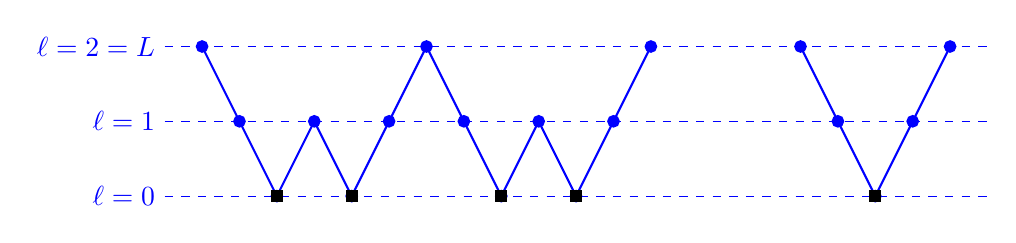
\begin{tikzpicture}[>=latex,scale=0.95]
      \draw[blue, dashed](-0.5,2) node[left]{$\ell=2=L$}--(10.5,2);
      \draw[blue, dashed](-0.5,1)node[left]{$\ell=1$}--(10.5,1);
      \draw[blue, dashed](-0.5,0)node[left]{$\ell=0$}--(10.5,0);
      \begin{axis}[anchor=origin,x=1cm, y=1cm,hide axis]
        \addplot [mark=*, color=blue,thick] table {
          0 2
          0.5 1 
          1 0
          1.5 1
          2 0
          2.5 1
          3 2
          3.5 1
          4 0
          4.5 1
          5 0
          5.5 1
          6 2
        };
      \end{axis}
      \foreach  \x  in {1,2,4,5}{
        \node[black] at (\x,0) {\pgfuseplotmark{square*}};
      }
      \begin{scope}[shift={(8,0)}]
        \begin{axis}[anchor=origin,x=1cm, y=1cm,hide axis]
          \addplot [mark=*, color=blue,thick] table {
            0 2
            0.5 1 
            1 0
            1.5 1
            2 2
          };
        \end{axis}
        \foreach  \x  in {1}{
          \node[black] at (\x,0) {\pgfuseplotmark{square*}};
        }
      \end{scope}
    \end{tikzpicture}
  \end{center}
  \caption[W- and V- Cycles.]{One full ($p=2$) W-Cycle (left) and one full V-Cycle (right) for three levels, $L = 2$.}
\end{figure}

